\begin{center}
    \begin{figure}[H]
        \centering

        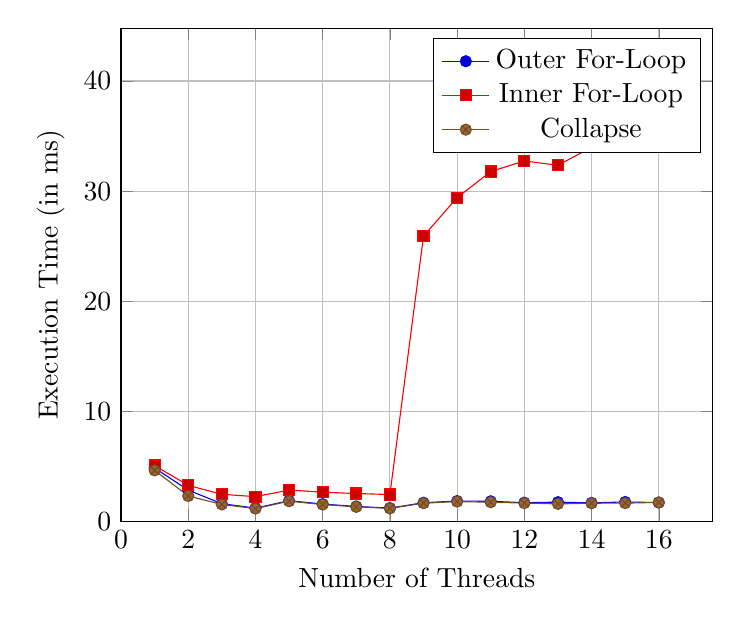
\begin{tikzpicture}
            \begin{axis}[
                title={},
                width=0.75\textwidth,
                xlabel={Number of Threads},
                ylabel={Execution Time (in ms)},
                xmin=0,
                ymin=0,
                grid=major
            ]
                \addplot coordinates {
                    (1,4.8388)(2,2.8324)(3,1.59845)(4,1.19935)(5,1.87025)(6,1.56525)(7,1.34835)(8,1.1991)(9,1.68795)(10,1.8391)(11,1.81815)(12,1.6916)(13,1.7405)(14,1.67545)(15,1.7581)(16,1.701)
                };
                \addlegendentry{Outer For-Loop}

                \addplot coordinates {
                    (1,5.06275)(2,3.26365)(3,2.45605)(4,2.23675)(5,2.84175)(6,2.64125)(7,2.52415)(8,2.43215)(9,25.9095)(10,29.4058)(11,31.7735)(12,32.7392)(13,32.3443)(14,33.981)(15,36.9086)(16,40.7253)
                };
                \addlegendentry{Inner For-Loop}       

                \addplot coordinates {
                    (1,4.6275)(2,2.3012)(3,1.5294)(4,1.153)(5,1.82735)(6,1.523)(7,1.31275)(8,1.1699)(9,1.64575)(10,1.7925)(11,1.73355)(12,1.65625)(13,1.58)(14,1.6422)(15,1.65035)(16,1.7164)
                };
                \addlegendentry{Collapse}
            \end{axis}
        \end{tikzpicture}
        \caption{Emboss Performance Tests dice.png}
    \end{figure}
\end{center}